
\chapter{Utilizzo di GDP - Gathering Detection Platform}\label{UtilizzoDiGDPGatheringDetecionPlatform}

\section{Pagina iniziale}\label{UtilizzoDiGDPGatheringDetecionPlatformPaginaIniziale}
La pagina iniziale che si presenta all'avvio è mostrata nella seguente figura.
Al suo interno sono presenti le componenti di seguito elencate e spiegate ognuna in una sezione a se stante.
\begin{enumerate}
	\item Il nome della web application$_{\scaleto{G}{3pt}}$;
	\item La barra di navigazione;
	\item Contenuto centrale;
	\item Il footer$_G$.
\end{enumerate}



\section{Barra di navigazione}\label{UtilizzoDiGDPGatheringDetecionPlatformBarraDiNavigazione}

La barra di navigazione è quella rappresentata in figura 3.1 dell'applicazione web$_{\scaleto{G}{3pt}}$. Tramite questa l'utente potrà navigare all'interno della piattaforma. Nella barra di navigazione sono presenti:
\begin{enumerate}
	\item \textit{Home}: link alla pagina iniziale;
	\item \textit{Chi siamo}: link alla pagina "Chi siamo";
	\item \textit{Barra di ricerca}: attraverso la barra di ricerca è possibile cercare, e quindi selezionare tra quelle disponibili, la città di cui si è interessati a visualizzare i dati sulla heat-map$_G$. 
\end{enumerate}
\begin{center}
	\begin{figure}
		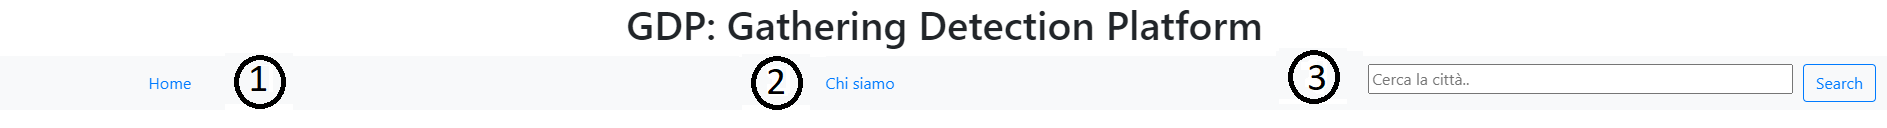
\includegraphics[width=1\linewidth]{../immagini/manualeUtente/BarraDiNavigazioe.png}
		\caption{Barra di Navigazione}
	\end{figure}
\end{center}
%scaricare il manuale utente ?????

\section{Contenuto centrale}\label{UtilizzoDiGDPGatheringDetecionPlatformContenutoCentrale}

\subsection{Pagina Iniziale - Home} \label{UtilizzoDiGDPGatheringDetecionPlatformContenutoCentralePaginaInizialeHome}
La pagina iniziale che visualizza l'utente è quella mostrata in figura n (quella che c'è sopra in 3.1). 


\subsubsection{Heatmap}\label{UtilizzoDiGDPGatheringDetecionPlatformContenutoCentralePaginaInizialeHomeHeatmap}
Al centro della web app$_{\scaleto{G}{3pt}}$ è presente una heat map$_{\scaleto{G}{3pt}}$ che raffigura, inizialmente, il flusso di persone presenti nella città di Roma nell'orario attuale. Successivamente l'utente potrà modificare la città, attraverso l'elenco delle città (\S~\ref{UtilizzoDiGDPGatheringDetecionPlatformContenutoCentralePaginaInizialeHomeMenùATendina}) oppure tramite la barra di ricerca, l'orario e la data, secondo quanto spiegato in \S~\ref{UtilizzoDiGDPGatheringDetecionPlatformContenutoCentralePaginaInizialeHomeCalendarioESlider}, e visualizzare tramite la heat map$_{\scaleto{G}{3pt}}$ i dati relativi ai campi selezionati.\\
Per facilitare la lettura della mappa, dopo che l'utente ha effettuato lo zoom-in$_G$, viene mostrato un pop-up$_G$, accompagnato da un marker$_G$, che evidenzia sia il nome del luogo che si sta osservando sia il numero di persone effettivamente presenti in quel momento. Questa funzionalità viene illustrata nella seguente figura n. (inserire figura pop-up)

\subsubsection{Elenco delle città} \label{UtilizzoDiGDPGatheringDetecionPlatformContenutoCentralePaginaInizialeHomeMenùATendina}
L'elenco delle città, posizionato a destra della mappa, viene utilizzato per la selezione della città. Infatti, l'utente, quando apre l'applicazione web$_{\scaleto{G}{3pt}}$, visualizza la mappa centrata sulla città di Roma, la città di default, ma successivamente può scegliere di osservare il flusso di persone relativo ad un'altra città presente tra quelle messe a disposizione nella lista. 
\begin{center}
	\begin{figure}
		\includegraphics[width=0.2\linewidth]{../immagini/manualeUtente/ElencoCittà.png}
		\caption{Elenco Città}
	\end{figure}
\end{center}

\subsubsection{Calendario e slider}\label{UtilizzoDiGDPGatheringDetecionPlatformContenutoCentralePaginaInizialeHomeCalendarioESlider}
L'utente ha a disposizione, a sinistra della mappa, un calendario che gli permette di scegliere l'anno, il mese ed il giorno di cui desidera visualizzare i dati. Per selezionare il mese bisogna spostarsi usando le freccie poste ai lati (1), mentre per l'anno si seleziona sull'anno corrente (2).
%da scrivere che può solo andare nel passato e presente?
\begin{center}
	\begin{figure}
		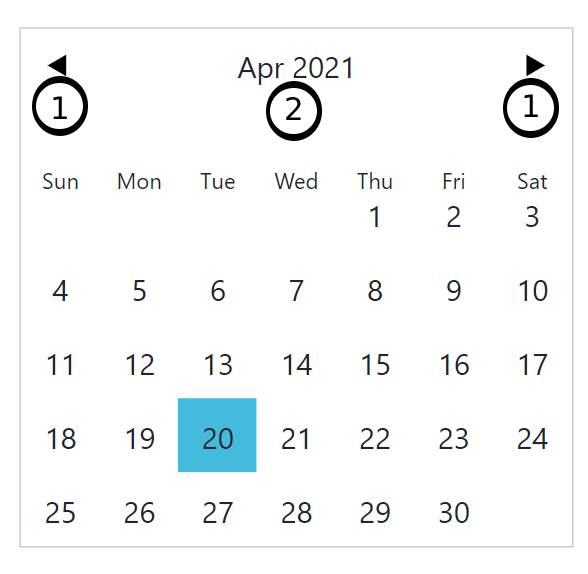
\includegraphics[width=0.3\linewidth]{../immagini/manualeUtente/Calendario.jpg}
		\caption{Calendario}
	\end{figure}
\end{center}
Al di sopra della mappa, invece, è presente uno slider$_G$ con il quale l'utente può scegliere un orario diverso da quello attuale di cui desidera visualizzare i dati attraverso la heat map$_{\scaleto{G}{3pt}}$. La selezione dell'orario è effettuata su intervalli di tempo di ora in ora. Per selezionare l'ora attravero lo slider, si può sia cliccare sulla scritta dell'orario che si vuole selezionare sia spostare il tooltip (non so come si chiami) (1).
\begin{center}
	\begin{figure}
		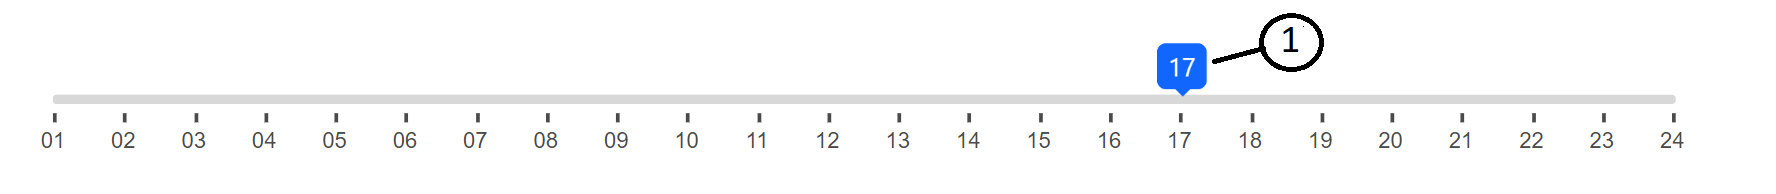
\includegraphics[width=1\linewidth]{../immagini/manualeUtente/Slider.png}
		\caption{Slider}
	\end{figure}
\end{center}

\subsubsection{Bottone Reload Map} \label{UtilizzoDiGDPGatheringDetecionPlatformContenutoCentralePaginaInizialeHomeBottoneReloadMap}
Nel caso in cui l'utente avesse selezionato una data diversa da quella odierna e/o un'ora differente da quella attuale, cliccando sul pulsante "Reload Map", la mappa si aggiornerà e tornerà a mostrare i dati in tempo reale, quindi relativi a data e ora corrente, rimanendo sulla città che si stava osservando. 
\begin{center}
	\begin{figure}
		
\includegraphics[width=0.3\linewidth]{../immagini/manualeUtente/ReloadMap.png}
		\caption{Reload Map}
	\end{figure}
\end{center}

\subsubsection{Messaggio d'errore} \label{UtilizzoDiGDPGatheringDetecionPlatformContenutoCentralePaginaInizialeHomeMessaggioDiErrore}
Nel caso in cui non ci siano dati disponibili nel database per il luogo, il giorno e l'ora in questione, l'utente visualizzerà un messaggio di errore che lo informerà del disguido e la mappa non mostrerà nessun dato. L'utente potrà chiudere il messaggio d'errore premendo il pulsante "OK". 
\begin{center}
	\begin{figure}
		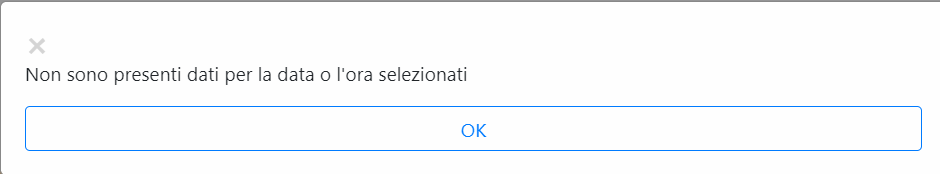
\includegraphics[width=0.5\linewidth]{../immagini/manualeUtente/MessaggioErrore.png}
		\caption{Messaggio d'errore}
	\end{figure}
\end{center}

\subsection{Chi siamo} \label{UtilizzoDiGDPGatheringDetecionPlatformContenutoCentraleChiSiamo}
(inserire immagine)\\
In questa pagina è possibile visualizzare le informazioni che riguardano il team di sviluppo \textit{Jawa Druids}, l'azienda proponente \textit{Sync Lab} e il progetto \textit{GDP: Gathering Detection Platform}. 
%da completare+
\begin{center}
	\begin{figure}
		
\includegraphics[width=0.5\linewidth]{../immagini/manualeUtente/AboutUs.png}
		\caption{Footer}
	\end{figure}
\end{center} 

\section{Footer}\label{UtilizzoDiGDPGatheringDetecionPlatformFooter}
Il footer$_{\scaleto{G}{3pt}}$ è presente in tutte le pagine dell'applicazione web$_{\scaleto{G}{3pt}}$ e riporta alcuni link utili, come quello del sito web dell'azienda \textit{Sync Lab} e la mail del team di sviluppo, da contattare in caso si riscontrino problemi con l'uso del prodotto software$_G$. 
%da sistemare
\begin{center}
	\begin{figure}
		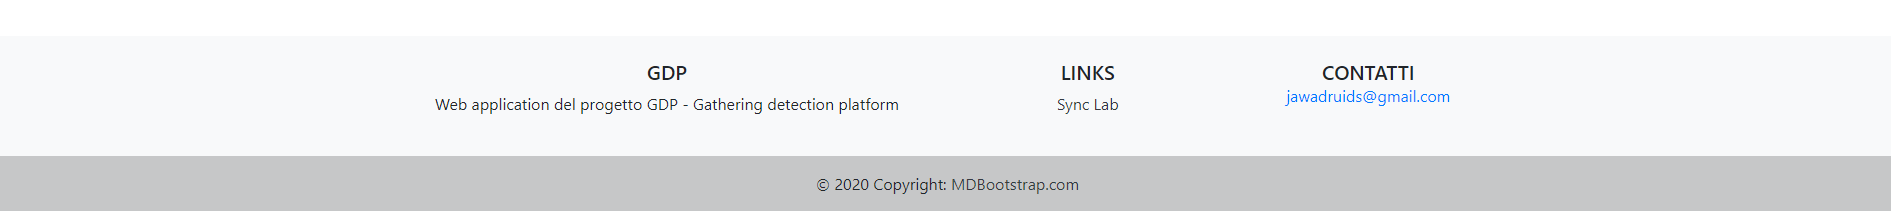
\includegraphics[width=1\linewidth]{../immagini/manualeUtente/Footer.png}
		\caption{Footer}
	\end{figure}
\end{center}


%COSE DA VALUTARE SE SCRIVERE O MENO
%1) che la mappa si aggiorna ogni 10 minuti automaticamente??? (ancora da implementare in realtà)
%2) parte di predizione?? slider +2 ore rispetto a quella attuale
